\Author{\daAuthorTwo}

Before even starting the development of our app, we decided to mock up the user interface. This turned out to be very helpful during implementation because we had an idea of how things should look and did not need to think about design choices while writing code. We used Figma to create these wireframes.

\blankLine

\subsection{Map View}

This map view is the center point of our app. Here, the addresses that still need to be visited get displayed, and comments can be added. The user can move, zoom, or rotate the map as well as click on markers to see details and edit the comment field. There are also visual indicators for addresses that are already commented, as well as different icons depending on the specification of an address. On the bottom of our app is a navigation bar that stays consistent across the different screens and is used to switch between them. Our primary goal was to keep the map as simple as possible to avoid distraction or overwhelming the user.

\begin{figure}[H]
    \centering
    \begin{minipage}{0.3\textwidth}
        \centering
        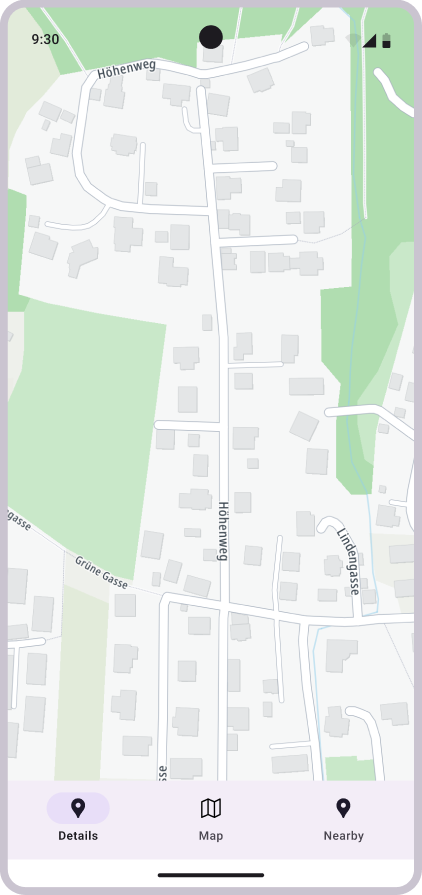
\includegraphics[width=\textwidth]{images/paul/wireframes/mapScreen.png}
        \caption{Initial wireframe}
    \end{minipage}
    \hspace{2cm}
    \begin{minipage}{0.3\textwidth}
        \centering
        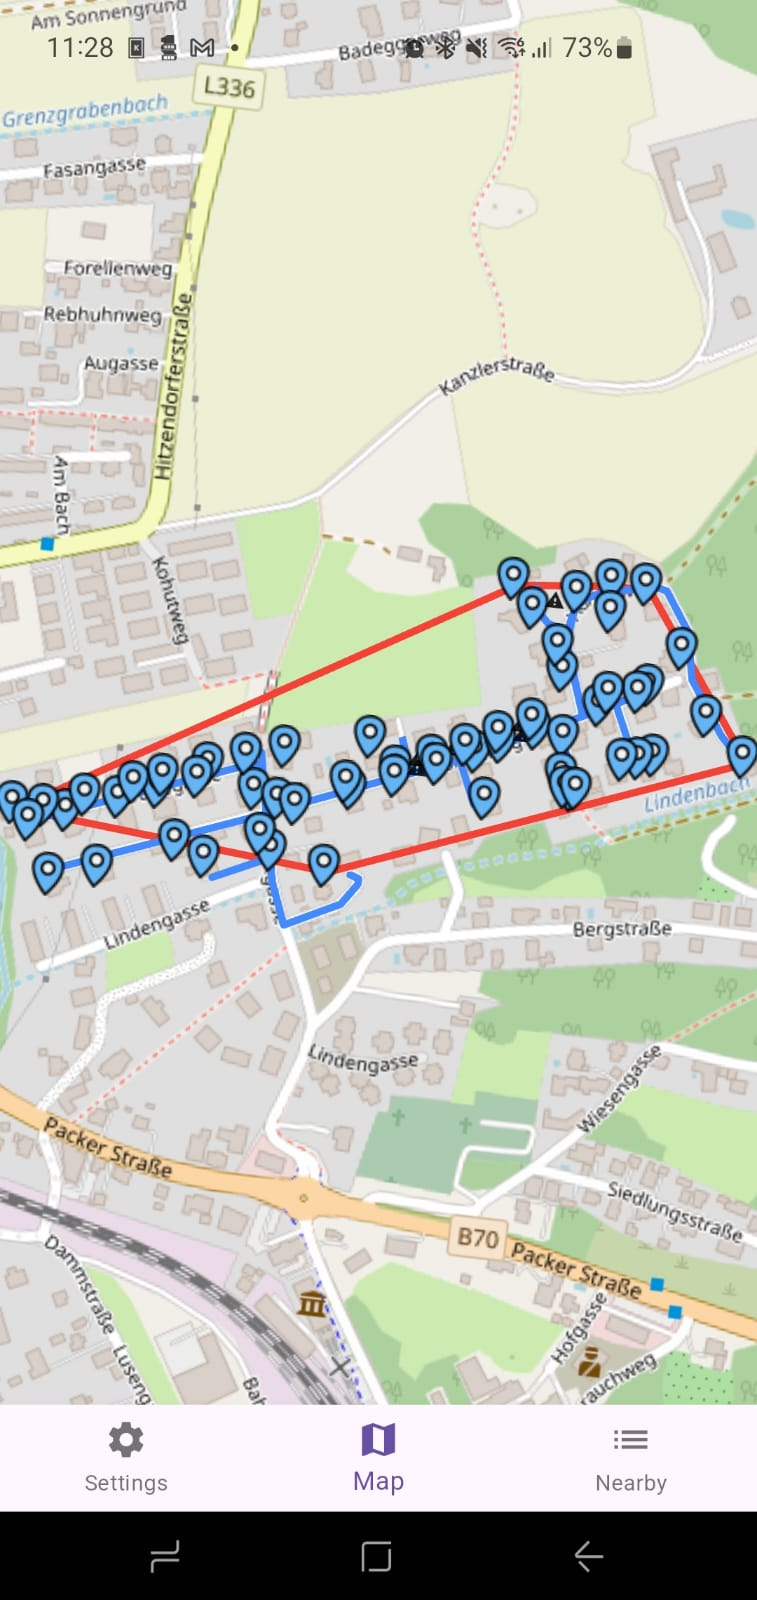
\includegraphics[width=\textwidth]{images/paul/wireframes/finalMap.jpeg}
        \caption{Final screen in app}
    \end{minipage}
\end{figure}

\subsection{List View}

This screen consists of a list in which all addresses that are in the selected area get displayed. They are grouped by the street and are sorted ascending by the house number. The user can swipe on either individual house items or the street name to change the \texttt{alreadyVisited} field. When swiping on a whole street, the user has to secondly approve that they really want to toggle all the addresses of this street. Initially it was planned to also incorporate the distance to a specific address into this list. This feature was later abandoned because of time constraints. 

\blankLine

There were two different ideas to integrate this view into the app. First, using a panel that can be pulled out of the right side of the screen, but during development, we chose to just make it its own page for a simpler-to-navigate experience. Also, the swipe gesture was added later, after the initial planning. In the wireframe, there were checkboxes that indicated the state.

\begin{figure}[H]
    \centering
    \begin{minipage}{0.26\textwidth}
        \centering
        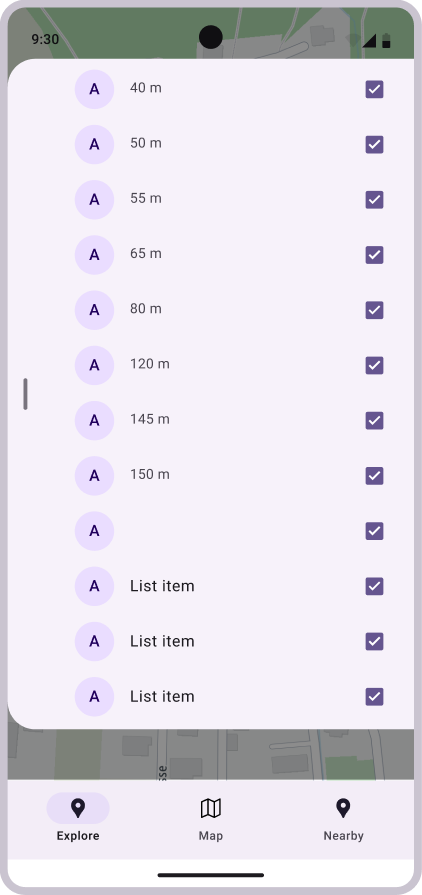
\includegraphics[width=\textwidth]{images/paul/wireframes/listScreenv1.png}
        \caption{Initial idea of List view with pull-out panel}
    \end{minipage}
    \hspace{0.3cm}
    \begin{minipage}{0.26\textwidth}
        \centering
        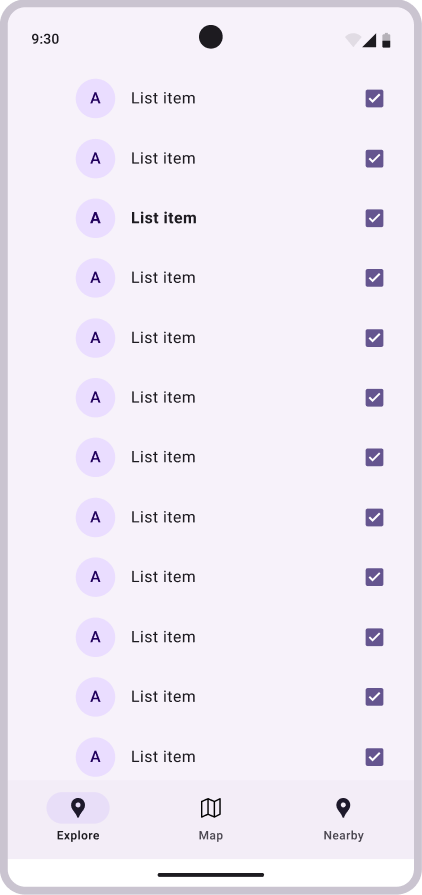
\includegraphics[width=\textwidth]{images/paul/wireframes/listScreenv2.png}
        \caption{List view with different opening concept}
    \end{minipage}
    \hspace{0.3cm}
    \begin{minipage}{0.26\textwidth}
        \centering
        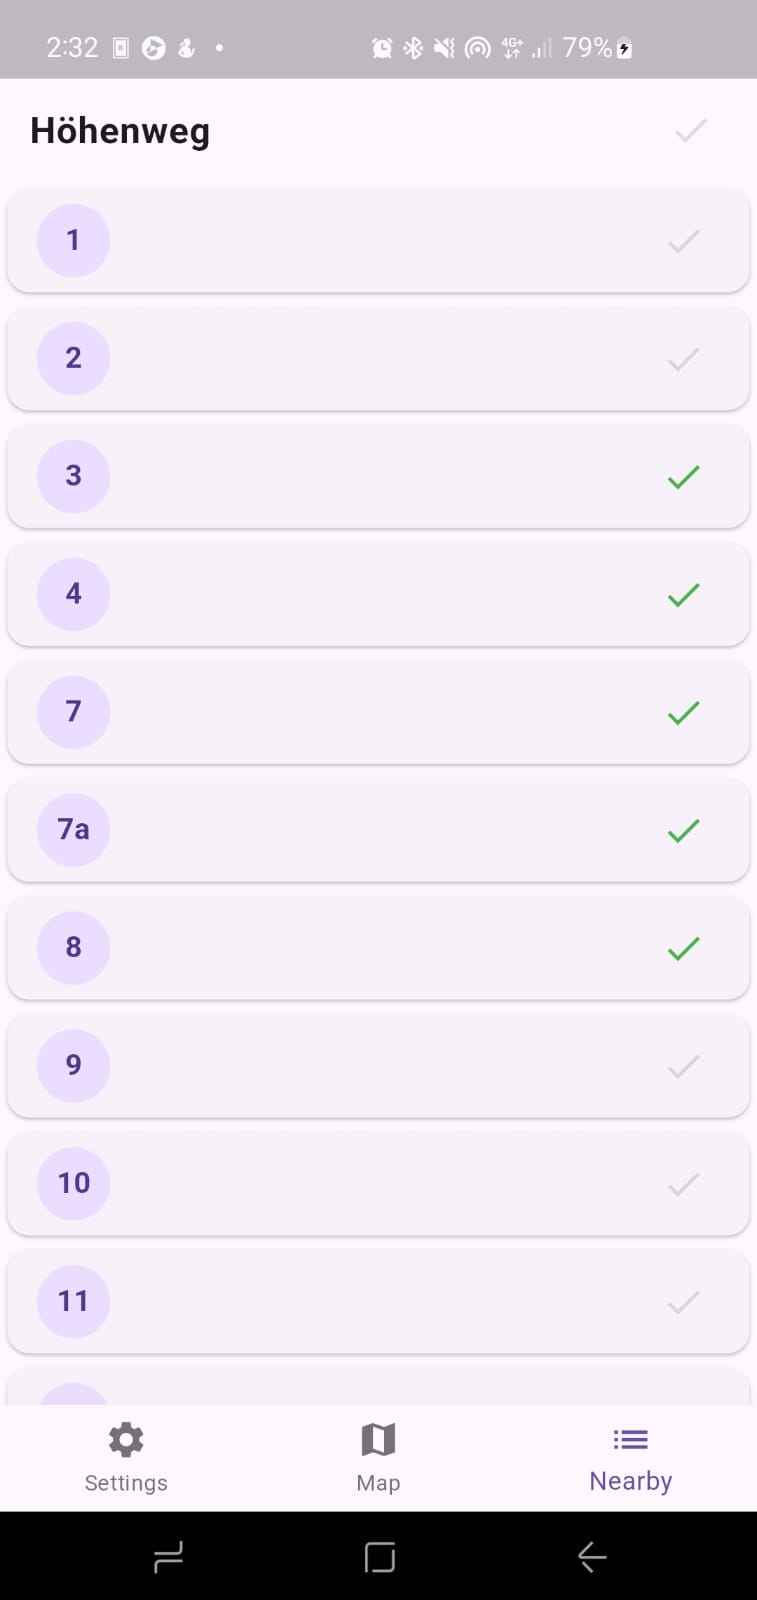
\includegraphics[width=\textwidth]{images/paul/wireframes/finalList.jpeg}
        \caption{Final implementation of List view with swipe gestures}
    \end{minipage}
\end{figure}

In the end, a few things changed, but the basic concept has stood since the project started.

\subsection{Details View}
This view was designed to not be a whole separate screen from the beginning, but it was basically completely reworked during development. At first, it was planned to be a sliding panel, just like the list view. It ended up being just a small pop-up that gets displayed when a user taps on a marker. In this dialog, the house number, street name, postal code and a text field for comments get displayed. Through two color-coded buttons, the comment can be either saved or discarded.

\begin{figure}[H]
    \centering
    \begin{minipage}{0.3\textwidth}
        \centering
        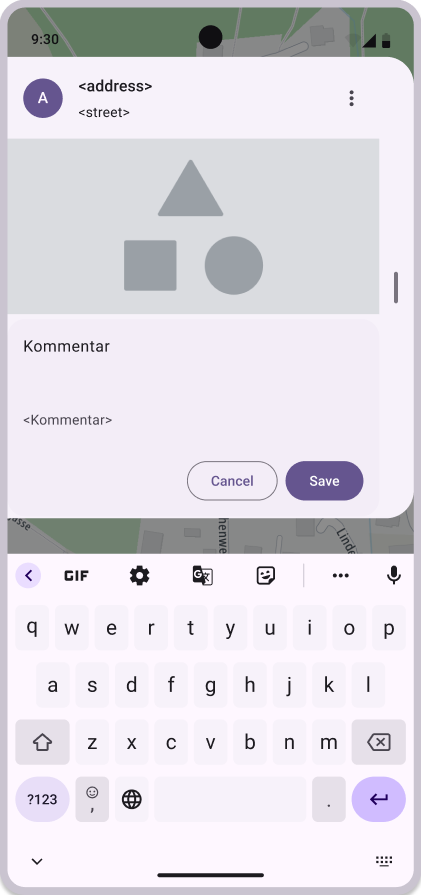
\includegraphics[width=\textwidth]{images/paul/wireframes/detailsScreen.png}
        \caption{Wireframe of map screen}
    \end{minipage}
    \hspace{2cm}
    \begin{minipage}{0.3\textwidth}
        \centering
        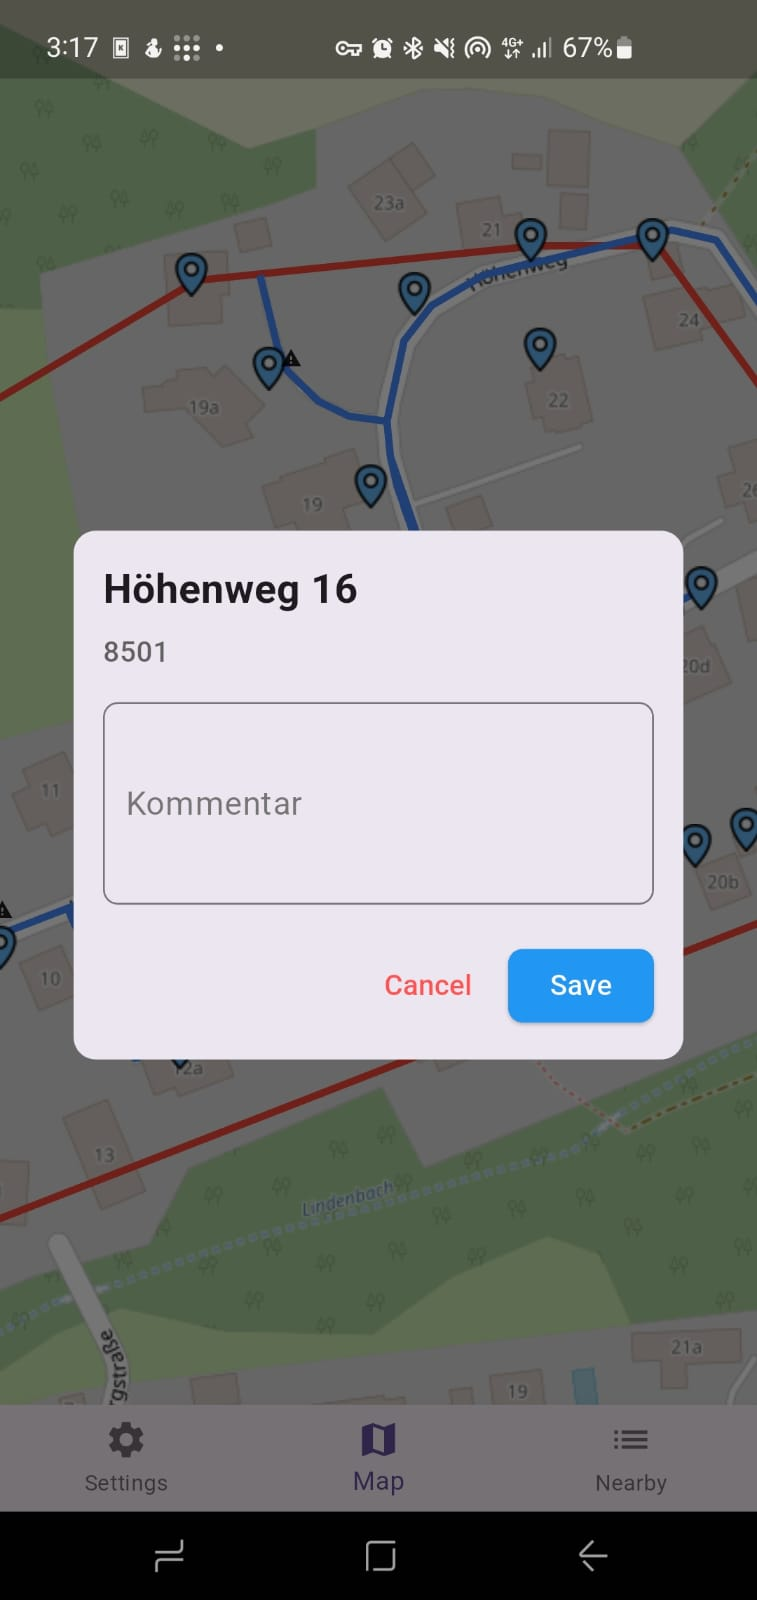
\includegraphics[width=\textwidth]{images/paul/wireframes/finalDetails.jpeg}
        \caption{Final version of map with markers}
    \end{minipage}
\end{figure}

\subsection{QR-Code Scanner}
This page was initially not planned or mocked up, since it was still unclear how a user would get their area assigned. Eventually we decided on QR-Codes for their ease of use. But to be able to scan the codes, which can be printed from the Admin Panel, we needed to implement a simple scanning mechanism. In the end, we created a single new page with just a button that starts the scanner. This page can and will be expanded in future releases to feature additional settings like an optional dark mode or user-changeable colors. 

\subsection{Possible improvements for future versions}

In a future iteration of the app, the details' dialog should be accessible from the list view, also, according to the feedback we got from legitimate users of our app, it would be nice to have more states than just visited or not. For example, visited, but nobody was home, will not visit again this year, or visited, somebody was at home, but wishes to not be visited anymore. To implement this, the entire list screen needs to be completely redesigned. Additionally, the feature that the user can see which address is closest to them would probably be useful. Furthermore, reliably displaying the user's current location would be appreciated.